\section{Introduction}

The recent success of large-scale machine learning models is fundamentally reshaping the computing landscape~\cite{hu2024characterization, choudhury2024mast, gangidi2024rdma, qian2024alibaba}. Training and serving large models require massive distributed GPU clusters: a fragile and resource intensive endeavor, highly susceptible to various hardware and software failures~\cite{megascale, gandhi2024recycle}. For example, pre-training of LLaMA3 on a cluster of 16,384 GPUs experienced 466 job interruptions during a 54-day training period~\cite{llama3} and the mean-time-to-failure was only 2.7 hours. Once a failure occurs, a noticeable recovery time is often required~\cite{unicron,megascale}.

While network communication is one of the key performance bottlenecks in ML training~\cite{Megascalemoe,zhou2025accelerating,wang2023zeroplusplus,song2023optimus}, network failures and interruptions remain an under-addressed source of inefficiency~\cite{wang2024towards, yu2023understanding, Revisiting_Reliability}.
Recent industry reports show that network issues are among the leading causes of job failures in large ML clusters~\cite{llama3, Revisiting_Reliability, liu2024hostmesh, wan2025robust}, and faults such as cable and NIC issues can account for up to half of all failed training jobs~\cite{unicron}. Similarly, these failures also affect inference systems, where even a single stalled collective can significantly increase tail latency or trigger costly request retries~\cite{ICML2024}. A key reason is that current collective communication libraries (CCLs), such as NCCL~\cite{NCCL}, are {\em fail-stop}: any network error aborts the communicator, crashes the process, and forces the entire job to restart.

To recover from failures, existing ML frameworks fall into one of two extremes: (1) A checkpointing-based recovery process requires a \textit{complete relaunch} of the framework to restore the model's state from storage, incurring substantial latency for failure detection, resource re-allocation, state reloading, and re-computation of iterations lost since the last checkpoint~\cite{bytecheckpoint,eisenman2022check,gupta2024just,mohan2021checkfreq,wang2023gemini}. Recent efforts~\cite{unicron,megascale} show that the recovery time from a single failure can reach 68 minutes, wasting large amounts of GPU time in jobs~\cite{wang2023gemini}. (2) An emerging response is to exclude the failed server node~\cite{oobleck,gandhi2024recycle}. When any failure occurs, the framework runtime removes that worker along with its GPUs, rebuilds the job, and communicates over the remaining ranks, thereby avoiding a full restart while still interrupting progress and reducing the effective usage of GPUs if only network issues are present.

From a systems layering perspective, these approaches are unsatisfactory because they handle network failures at the application (ML framework) layer rather than within the communication layer. Analogous to how transport protocols such as TCP provide reliability for packet loss~\cite{saltzer1984end,zimmermann1980osi}, the CCL layer should itself offer a more \textit{resilient} abstraction under network faults. In other words, there ought to be a \textit{middle ground} in which the CCL transparently routes around transient link and NIC failures, degrades gracefully, and exposes meaningful signals to guide higher-level recovery decisions.

One opportunity to improve CCL resilience in modern multi-NIC GPU clusters is the increasing heterogeneity of network link types between GPUs (e.g., PCIe and NVLink), which creates potentially redundant network paths for communication, even if some of these paths may fail. In this paper, we want to explore whether there are alternative cases in which
\textbf{\textit{CCL layer can exploit the path redundancy to continue the ongoing job efficiently rather than giving up immediately.}}

In this paper, we present R2CC, a reliable and resilient collective communication library that transforms collective communication from fail-stop to fail-operational under inter-node network failures (Figure~\ref{fig:r2ccandnofailure}). When a NIC or link fails but alternative paths remain available, R2CC detects faults during ongoing collectives, migrates in-flight transfers losslessly to healthy connections, and adapts collective schedules to the degraded topology. As a drop-in extension for NCCL~\cite{NCCL}, R2CC requires no framework changes for transparent repair and optimization. R2CC additionally exposes degradation signals, reporting failure location and bandwidth loss, enabling frameworks that integrate with R2CC to make informed policy decisions on continuation, checkpointing, or recovery. To realize this, we address the following key challenges.

{\bf \#1: How to detect and locate the failure in an ongoing collective operation (e.g., AllReduce)?} Detecting and pinpointing failures during an ongoing collective is difficult due to limited error visibility in RDMA. R2CC introduces bilateral failure awareness using an out-of-band notification path combined with probe-based RDMA fault localization.

{\bf \#2: How to losslessly migrate the failed connection to another connection via alternative links?} R2CC performs live migration to alternative paths using two techniques. First, \textit{eager provisioning} multi-registers GPU buffers with local NICs and pre-establishes backup RDMA connections to neighboring servers at initialization. Second, \textit{protocol-aware suffix replay} reconciles a conservative replay boundary with the peer over the out-of-band channel, so the collective can safely replay only the unfinished suffix on the backup connection under both throughput-oriented and low-latency CCL protocols.
These techniques allow collectives to resume seamlessly on a backup NIC.

{\bf \#3: How to perform failure-aware collective online optimization  with single or multiple failures?} R2CC selects from several failure-aware optimizations. \textit{R2CC-Balance} redistributes traffic across remaining NICs (PCIe-, NUMA-, and PXN-aware) for all collectives. \textit{R2CC-AllReduce} modifies the AllReduce schedule to reduce the workload on the degraded server, combining global and partial AllReduce operations. Third, for multi-failure scenarios, an extended topology-aware \textit{recursive R2CC-AllReduce} can navigate bandwidth asymmetry and rail mismatches.

We evaluate R2CC on a testbed consisting of four NVIDIA DGX servers, each equipped with 8$\times$H100 GPUs and 8 InfiniBand 400Gbps NICs. We complement this with large-scale simulations using the state-of-the-art training simulator SimAI~\cite{wang2025simai} to model clusters of up to 1024 GPUs under diverse failure patterns.
With a single NIC failure injected (i.e., a 12.5\% bandwidth loss in the affected server), our experiments show that R2CC incurs less than 1.1\% overhead for training and less than 3\% for inference. Compared with recent fault-tolerant systems for training and inference, R2CC achieves up to 92\% and up to 98\% lower overheads respectively.

\begin{figure}[t]
    \centering
    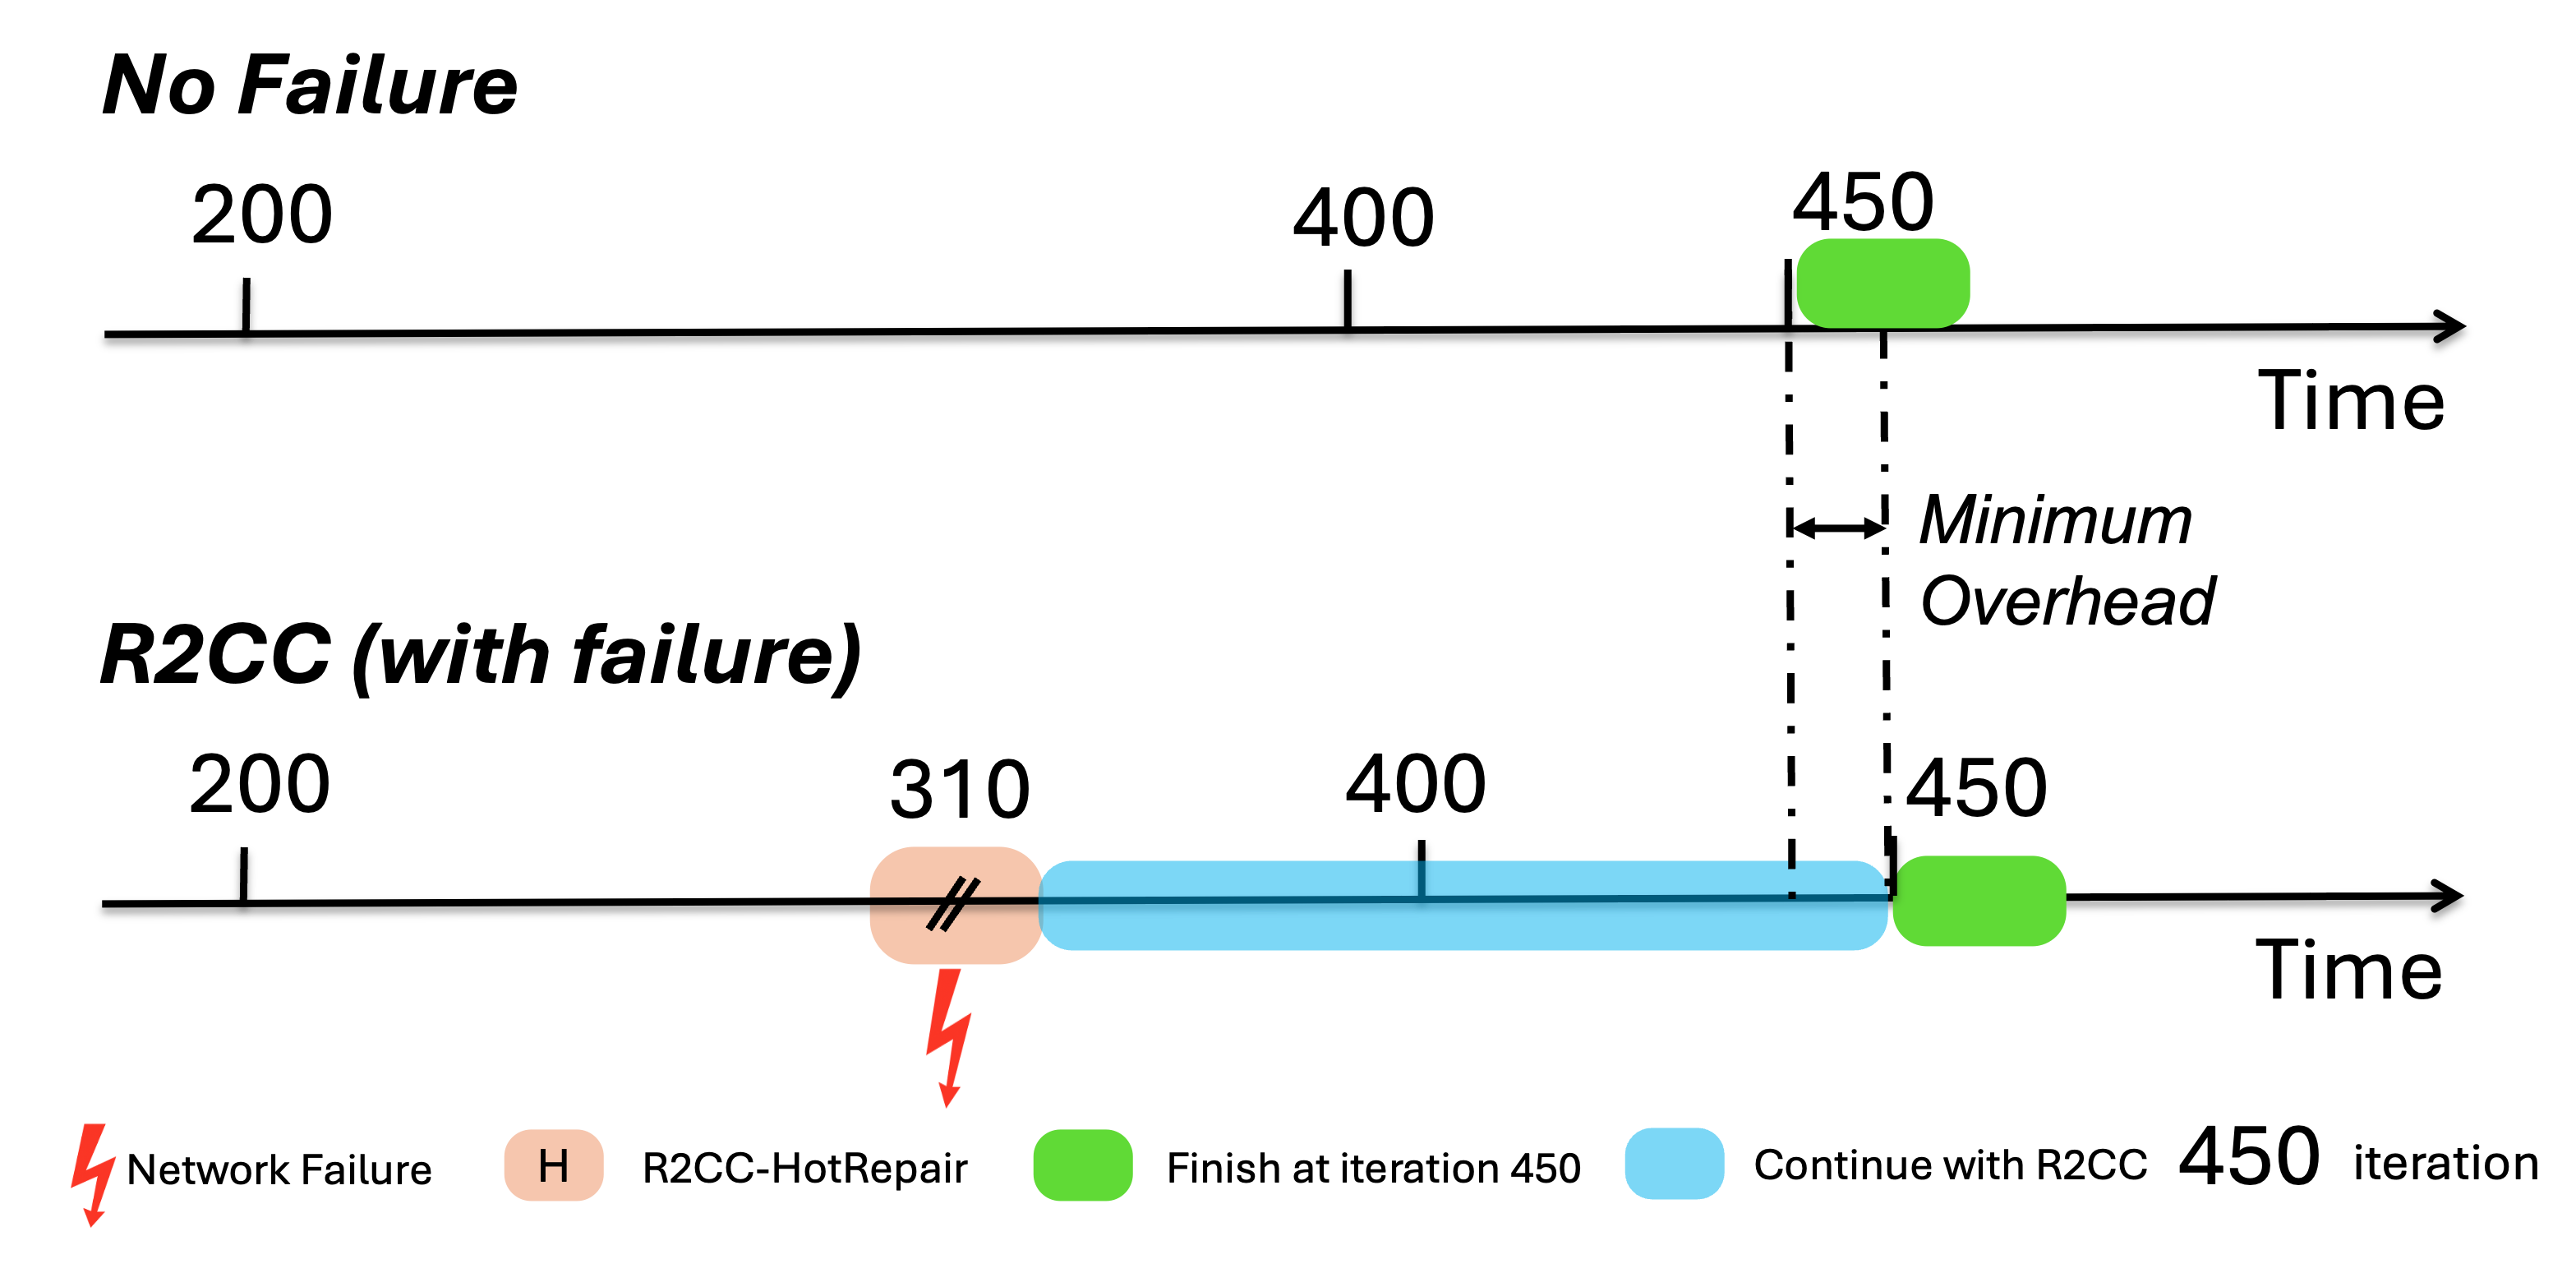
\includegraphics[width=0.95\columnwidth]{figs/new-first.png}
    \vspace{-2mm}
\tightcaption{\textbf{R2CC (with failure) vs. Ideal (failure-free)}}
    \label{fig:r2ccandnofailure}
    \vspace{-2mm}
\end{figure}
